\chapter{Artificial Neural Nets - Supervised Learning: Classification }
% Authors: Colin Andrus , Aakriti Gupta, Daniel Rivera, 2/11/18.

\section{Example of Not Linearly Separable Curves}

We have three curves defined by functions:
\[X_c(t) = t
\begin{pmatrix}
    \sin( \frac{2 \pi}{C}(2t + c -1)) \\
    \cos( \frac{2 \pi}{C}(2t + c -1))
\end{pmatrix}
 \]
\[ 0 \leq t \leq 1 \quad c = 1,..., C\]

\begin{figure}[ht]
    \centering
    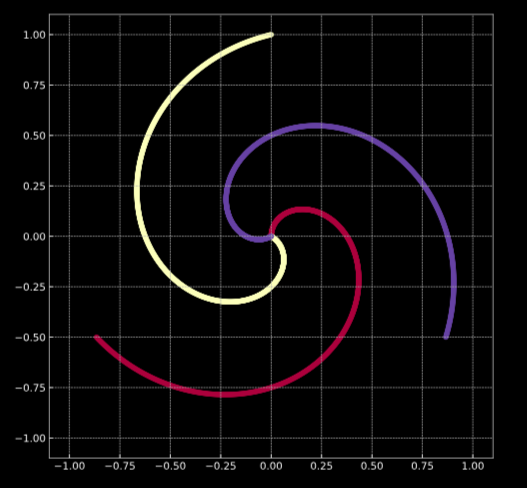
\includegraphics[width=200pt]{figs/spiral1.png}
    \caption{3 not linearly separable parametric curves}
    \label{fig:spiral}
\end{figure}
 
\newpage

If we were to use two linear transformations $ W_h$ and $ W_y$  transform the data $x$ as so:
\[\matr{h}= \matr{W_h}\matr{x}+ \vect{b_h} \]
\[\hat{\vect{y}} = \matr{W_y} \matr{h} + \vect{b_y}\]
we would not be able to  linearly separate the data points in these curves as shown in \cref{fig:spiral_with_noise}.
These points are defined by the same function with added noise.

\[X_c(t) = t
\begin{pmatrix}
    sin( \frac{2 \pi}{C}(2t + c -1) + \mathcal{N} (0, \sigma ^2 )) \\
    cos( \frac{2 \pi}{C}(2t + c -1) + \mathcal{N} (0, \sigma ^2 ) )
\end{pmatrix}
 \]
\[ 0 \leq t \leq 1 \quad c = 1,..., C\]

\begin{figure}[ht]
    \centering
    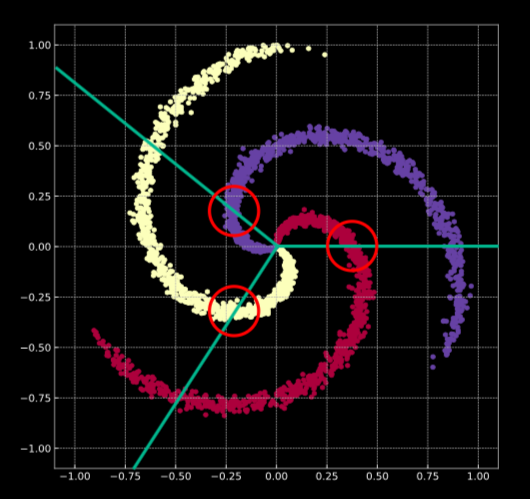
\includegraphics[width=200pt]{figs/spiral2.png}
    \caption{These data points of three different classes (represented by color) generated from curves with added noise cannot be separated only with linear functions.}
    \label{fig:spiral_with_noise}
\end{figure}

In this case, the best a classifier consisting of solely linear layers can do is to rotate the decision boundaries centered around the origin to predict slightly more than half of the data points correctly as shown in \cref{fig:spiral_linear_classifier}.
We are limited to only the linear transformations of rotations, scaling and shearing.
We are not able to "warp" the data in the higher dimensional space used in our linear layers to allow for separation in that higher dimension without a non-linear activation function.

\begin{figure}[ht]
    \centering
    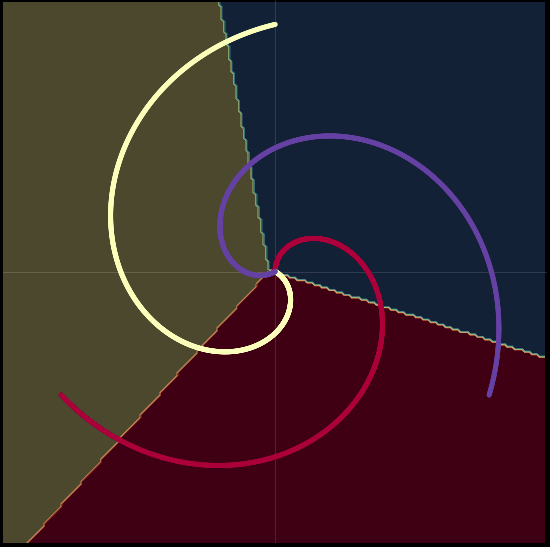
\includegraphics[width=200pt]{figs/linear.png}
    \caption{2 linear layers alone cannot create a classifier that performs well for this data}
    \label{fig:spiral_linear_classifier}
\end{figure}

To improve the accuracy of the classifier, we introduce the non-linear functions $f$ and $g$ resulting in the 3-layer architecture depicted in \cref{fig:3-layer_arch}.
Common selections for these functions include ReLU, tanh, sigmoid and softmax.
Finally, the equations that define the network are as follows:
\begin{align*}
    \vect{h} &= f(\matr{W}_{\vect{h}}\vect{x} + \vect{b}_{\vect{h}}) \\
    \hat{\vect{y}} &= g(\matr{W}_{\vect{y}}\vect{h} + \vect{b}_{\vect{y}})
\end{align*}

\begin{figure}[ht]
    \centering
    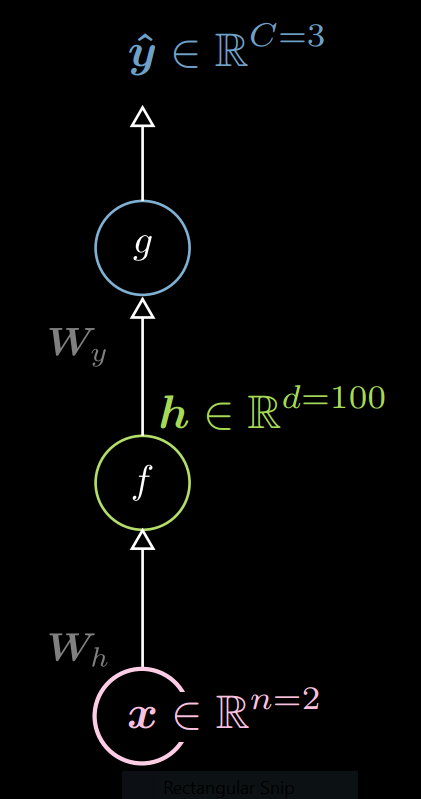
\includegraphics[width=100pt]{figs/architecture.png}
    \caption{Architecture of the 3-layer ANN used for the spiral classification problem, where $f$ and $g$ are non-linear functions.}
    \label{fig:3-layer_arch}
\end{figure}

where $\vect{x} \in \mathbb{R}^n$, $\vect{h} \in \mathbb{R}^d$ and $\hat{\vect{y}} \in \mathbb{R}^C$.
For the current example, the input space is two-dimensional ($n=2$), the hidden high-dimensional space has $d=100$ and the output space has $C=3$ (the number of classes of the original classification problem).
The dimension of the hidden space for this examples satisfies $d >> n$, which spreads the data points making them easier to manipulate and separate than in the original low-dimensional input space.

The dimensions of the weight matrices and bias terms must be selected so as to be consistent with these definitions, thus $\matr{W}_{\vect{h}} \in \mathbb{R}^{d \times n}$, $\matr{W}_{\vect{y}} \in \mathbb{R}^{C \times d}$, $\vect{b}_{\vect{h}} \in \mathbb{R}^d$ and $\vect{b}_{\vect{y}} \in \mathbb{R}^C$.

It is worth noticing that for each non-linearity there is an associated affine transformation, characterized by a rotation $\matr{W}\vect{x}$ and a translation $\vect{b}$.


\subsection{2 Ways to View Neural Nets}
When diagramming or describing a neural network, we begin with the input data at the bottom and then build up with our linear and non-linear transformations to the output at the top. With this structure defined, there are 2 ways to view the behavior of a model (\cref{fig:views}):\\

\begin{enumerate}
    \item \textbf{Bottom Up}\\
    Looking up at the original data with decision boundary that has been warped by the model.
    \item \textbf{Top Down}\\
    Looking down at data that has been warped by the model.
\end{enumerate}

\begin{figure}[ht]
    \centering
    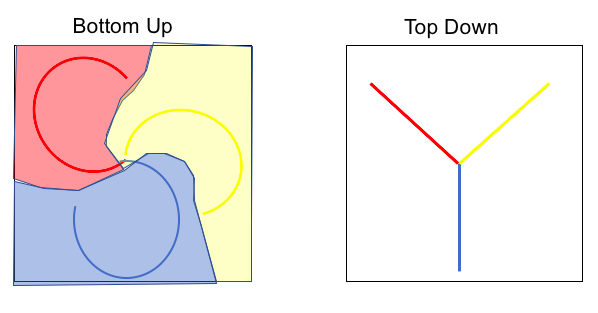
\includegraphics[width=300pt]{figs/views.png}
    \caption{Sketches of the two ways of viewing a Neural Net: bottom up (left) and top down (right).}
    \label{fig:views}
\end{figure}

\subsection{Output 1-hot encoding} \label{ssc:1hot}
In our previous example, the most straightforward way to map the categorical labels \{Red, Green, Blue\} into numerical values would be to simply assign a number to each color, \emph{i.e.}\ \{Red=1, Green=2, Blue=3\}.
However, this approach is not compatible with the softmax function that is typically used for classification problems, which assigns probability-like scores between 0 and 1 to each category. 

Furthermore, using natural numbers introduces a notion of distance or proximity that is not really present in the original categorical data.
For instance, one could be inclined to think that Blue is more similar to Green than it is to Red because 3 is closer to 2 than it is to 1.
The truth is, however, that all three categories are equally dissimilar and this notion of distance does not exist among them.

To avoid this problem and to conform to the output generated by the softmax layer, we encode the labels using a technique known as \emph{1-hot encoding}.
For a classification problem with $C$ classes, each class will be mapped to a unit vector in $\mathbb{R}^C$. The vector corresponding to the $i$-th class in the original problem will have a $1$ in its $i$-th dimension and $0$'s elsewhere (hence the name 1-hot encoding).

Applying this to the problem at hand we have Red = $(1,0,0)$, Green = $(0,1,0)$ and Blue = $(0,0,1)$.

\subsection{Neural Network Training: Part 1}
The last layer of a neural network trained for a classification problem is usually a softmax function, which is defined as follows:

\begin{equation*}
    \hat{\vect{y}}[c] = \text{softmax}(\vect{l})[c] = \frac{\exp(\vect{l}[c])}{\sum_{j=1}^C \exp(\vect{l}[j])} \in (0,1)
\end{equation*}

Where $\vect{l}$ is the \emph{logits} vector of raw (non-normalized) predictions that the classification model generates, which is then passed to the normalization function, \emph{i.e.}\ softmax.
The notation $[c]$ refers to the $c$-th element of the vector, which leads us to conclude that $c \in [0,C-1]$ according to the 1-hot encoding described in \cref{ssc:1hot} and considering a 0-indexed vector (as it is the default and standard in Pytorch).

Given the index $c$ in the 1-hot encoding representation of the correct label and the vector of probabilities $\hat{\vect{y}}$ returned by the model, we can define the \emph{cross-entropy} or \emph{negative log-likelihood} loss as follows:

\begin{align*}
    \ell(\hat{\vect{y}},c) &= -\log(\hat{\vect{y}}[c]) \\
    \mathcal{L}(\hat{\vect{Y}},\vect{c}) &= \frac{1}{m}\sum_{i=1}^m \ell(\hat{\vect{y}}^{(i)},c^{(i)})
\end{align*}
Since the softmax produces exponentiation of the logits, we never receive exactly $0$ or $1$. Instead, $0^+$ or $1^-$ are returned which signify slightly greater than $0$ and slightly less than $1$.
Since the loss is the cross entropy/negative log of the output, if the correct class is predicted the loss will be $-\log(1^-)$, which is $0^+$. Similarly, for the other class $-\log(0^+)$ will be $+\infty$.

\subsection{Neural Network Training: Part 2}
Finally, How to train the Neural Network. 
\[\Theta \equiv \{ W_h, b_h , W_y, b_y \} \]
Here $\Theta$ is  a conglomeration of all the parameters and it represents one point in the parameter space.  
\[
   \mathcal{J}(\Theta) \equiv \mathcal{L}(\hat{\mathcal{Y}}(\Theta,c) \in R^+\
\]
$J(\Theta)$ is the loss over the entire data set and is a function of the parameter $\Theta$.

The next step is to compute the partial derivatives of the loss $\mathcal{J}(\Theta)$ with respect to the two different linear transformations. 
\[\matr{h} = f(\matr{W_h} \matr{x} + \vect{b_h})\]
\[\matr{\hat{y}} = f(\matr{W_y} \matr{x} + \vect{b_y})\]

Using backpropagation we find these two partial derivatives:
\[
    \frac{\partial J(\Theta)}{\partial \matr{W_y}} = 
    \frac{\partial J(\Theta)}{\partial \hat{\vect{y}}}
    \frac{\partial \hat{\vect{y}}}{\partial \matr{W_y}}
\]
    
\[
\frac{\partial J(\Theta)}{\partial \matr{W_h}} =
\frac{\partial J(\Theta)}{\partial \hat{\vect{y}}}
\frac{\partial \hat{\vect{y}}}{\partial \matr{h}}
\frac{\partial \matr{h}}{\partial \matr{W_h}}
\]


\begin{figure}[ht]
    \centering
    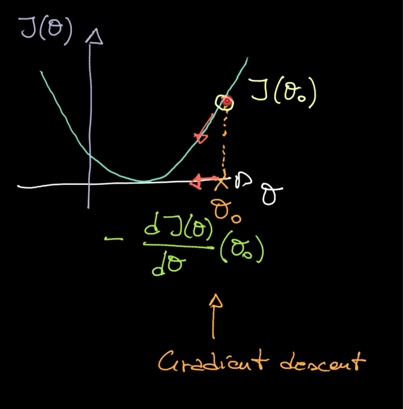
\includegraphics[width=300pt]{figs/gradient_descent.jpg}
    \caption{Representation: Gradient Descent}
    \label{fig:gradient_descent}
\end{figure}

Here $J(\Theta)$ is a  quadratic function, and given a point, the derivative/slope can be computed.
Let $\Theta_0$ be the starting position, the loss can be evaluate over the data set and the derivative or the slope can be figured out.
The derivative of $J(\Theta)$ which is a quadratic function will be a linear function.
In (\cref{fig:gradient_descent}) the slope at point $\Theta_0$ is positive, hence the derivative is linear function which points $\nearrow$, hence, weights will be modified by stepping in the opposite direction $\swarrow$.